\documentclass[tikz,border=2pt]{standalone}
\usepackage{amsmath,amssymb}
\usepackage{tikz}

\begin{document}
% x1 + x2 must equal 3, 5 or 8: binary selectors y1, y2, y3 with y1 + y2 + y3 = 1 pick one of
% the listed values; a fractional relaxation would allow everything in between.
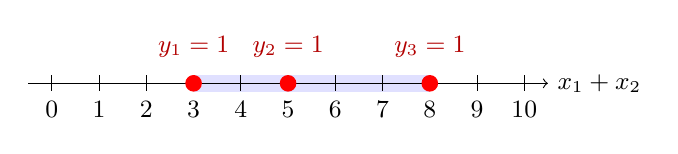
\begin{tikzpicture}[every node/.style={font=\small}]
	\draw[line width=6pt, blue!12] (1.8,0) -- (4.8,0);
	\draw[->] (-0.3,0) -- (6.3,0) node[right] {$x_1+x_2$};
	\foreach \x in {0,...,10} {\draw ({0.6*\x},0.1) -- ({0.6*\x},-0.1) node[below] {$\x$};}
	\fill[red] (1.8,0) circle (3pt); \fill[red] (3.0,0) circle (3pt); \fill[red] (4.8,0) circle (3pt);
	\node[red!70!black, anchor=south] at (1.8,0.2) {$y_1=1$};
	\node[red!70!black, anchor=south] at (3.0,0.2) {$y_2=1$};
	\node[red!70!black, anchor=south] at (4.8,0.2) {$y_3=1$};
	\end{tikzpicture}
\end{document}
